% Die vorangehenden fachlichen Kapitel 2 und 3 sind im aktuellen Template noch nicht angelegt.
% Der Zähler stellt vorläufig die vorgegebene Kapitelnummer her und ist nach der Integration der Kapitel 2 und 3 zu entfernen.
\setcounter{section}{3}
\section{Konzeption des IFC-basierten Annotationsmodells}\label{sec:ifc-annotationsmodell}

\subsection{Modellierungsziele und zentrale Designentscheidungen}\label{subsec:modellierungsziele-annotationsmodell}

Ein geometrisches Gebäudemodell beschreibt Form, räumliche Anordnung und fachliche Eigenschaften von Bauwerksobjekten,
enthält damit jedoch noch keine ausführbare Robotermission. Für die Missionsbeschreibung muss zusätzlich festgelegt
werden, welche Roboteraufgaben zu einem gemeinsamen Ziel gehören, welche konkrete Roboteraktion innerhalb einer Aufgabe
auszuführen ist und auf welche Gebäudeobjekte sich diese Aktion bezieht. Ferner sind Abhängigkeiten zwischen Aufgaben,
aktionsspezifische Parameter und gegebenenfalls Zeit- oder Planungsinformationen abzubilden. Die bloße Verknüpfung einer
Aufgabe mit einem IFC-Objekt genügt hierfür nicht. Insbesondere ist die Position eines referenzierten Objekts nicht ohne
Weiteres ein geeignetes Navigationsziel: Ein Türblatt kann beispielsweise das semantische Ziel einer Öffnungsaufgabe
sein, während die ausführbare Anfahrpose außerhalb seines Kollisionsraums liegen muss. Das Annotationsmodell muss daher
fachliche Referenzen und für die Ausführung erforderliche räumliche Ableitungen unterscheidbar halten.

Aus diesem Modellierungsproblem ergeben sich mehrere projektbezogene Ziele. Das Modell soll Robotermissionen semantisch
repräsentieren, Roboteraufgaben stabil mit IFC-Objekten verknüpfen und die Hierarchie der Aufgaben ebenso wie ihre
Ausführungsabhängigkeiten explizit erfassen. Es soll unvollständige oder widersprüchliche Missionen durch prüfbare
Regeln erkennbar machen und sich um weitere Aktionsarten sowie deren Parameter erweitern lassen. Zugleich soll es die
missionsbezogenen Angaben in annotierten IFC-Dateien persistierbar und austauschbar machen, ohne die Fachsemantik an die
Bedienoberfläche oder an einzelne Serialisierungsoperationen zu binden. Roboterspezifische Austauschformate werden aus
diesem fachlichen Bestand abgeleitet; sie bilden nicht selbst die maßgebliche Quelle des Projekts. Diese Zielsetzung ist
eine Modellierungsentscheidung der vorliegenden Arbeit und keine allgemeine Anforderung des IFC-Standards.

Eine zentrale Entscheidung betrifft den Träger der Aktionssemantik. Ein IFC-Gebäudeobjekt beschreibt, um welches
Bauwerksobjekt es sich handelt; eine konzeptionell vorgesehene Annotation von Objektfähigkeiten könnte ergänzen, welche
Interaktionen mit diesem Objekt grundsätzlich möglich sind. Demgegenüber legt eine Roboteraufgabe fest, welche konkrete
Aktion in einer bestimmten Robotermission ausgeführt werden soll. Deshalb wird die Aktionssemantik primär der Aufgabe
und nicht dem Zielobjekt zugeordnet. Dieselbe Tür kann dadurch in einer Aufgabe mit \texttt{OPEN} und in einer späteren
Aufgabe mit \texttt{CLOSE} verknüpft werden, ohne widersprüchliche Zustandsanforderungen am Tür-Objekt zu hinterlegen.
Die im Projekt verwendeten Werte \texttt{OPEN}, \texttt{CLOSE}, \texttt{SWITCH\_ON}, \texttt{SWITCH\_OFF},
\texttt{MOVE}, \texttt{PASS\_THROUGH} und \texttt{NAVIGATE\_TO} bilden ein projektspezifisches Aktionsvokabular; sie
sind keine
standardisierte IFC-Aufzählung. Das prototypisch implementierte Domänenmodell hält Vorbedingungen, Nachbedingungen,
benötigte Fähigkeiten und Erfolgskriterien als taskbezogene Felder vor.

Für Bearbeitung und Prüfung wird die Fachsemantik in einem eigenen internen Domänenmodell geführt. Der konzeptionelle
Datenfluss lautet: annotierte IFC-Datei, IFC-Import und Rekonstruktion, internes Domänenmodell, Bearbeitung und
Validierung sowie anschließend IFC-Mapping und Export. Das Domänenmodell stellt Missionen, Aufgaben, Aktionen,
Objektbezüge, Abhängigkeiten und optionale Zeitangaben in einer für Fachregeln geeigneten Form bereit. Die
IFC-Repräsentation dient dagegen der dauerhaften Speicherung und dem Austausch; eine Mapping-Schicht übersetzt
kontrolliert zwischen beiden Darstellungen. Zustände der Bedienoberfläche, etwa eine aktuelle Auswahl oder ein
geöffnetes Formular, sind davon zu trennen. Auch ausschließlich lokale UI-Angaben dürfen nicht unbemerkt zur fachlichen
Wahrheitsquelle werden. Diese Schichtung verhindert, dass IFC-Entitäten unmittelbar als veränderlicher UI-Zustand
behandelt werden, und ermöglicht Validierung unabhängig vom Rendering.

Am untersuchten Viewer-Stand ist diese Trennung prototypisch umgesetzt. Das interne, in TypeScript definierte Modell
unterscheidet Robotermission, Roboteraufgabe, Aktionsparameter, Objektbezug, Sequenz und Zeitangaben; gesonderte
Komponenten validieren das Modell und bilden es auf IFC-bezogene Records ab. Für direkt geladene IFC-Dateien existiert
außerdem eine Rekonstruktion der projektspezifischen Annotationen von Robotermissionen. Beim Export werden diese
Annotationen geschrieben, erneut importiert und semantisch mit dem beabsichtigten Domänenzustand verglichen. Dieser
Nachweis gilt nicht für beliebige strukturelle Änderungen eines IFC- oder Fragments-Modells und begründet daher keinen
allgemeinen vollständigen IFC-Roundtrip. Ein reines Fragments-Modell bleibt in diesem Ablauf ohne zugehörige
IFC-Quelldaten auf die Darstellung beschränkt.\footnote{Geprüfter Implementierungsstand: Viewer-Repository
\url{https://github.com/Tobilan/poc_thatopen}, Commit
\href{https://github.com/Tobilan/poc_thatopen/commit/674ede3bf2e7e6cf466bc4c16fe06c90fbb1753c}{\texttt{674ede3}}.
Relevante Pfade sind \path{src/domain/robot-tasks/types.ts}, \path{src/domain/robot-tasks/validation.ts},
\path{src/ifc/robot-tasks/mapper.ts}, \path{src/ifc/model-import/webIfcMissionReader.ts} und
\path{src/ifc/model-roundtrip/ifcMissionRoundtripCoordinator.ts}; zugehörige Testfälle liegen unter
\path{test/robot-tasks/}.}

Für den weiteren Entwurf wird die annotierte IFC-Datei als kanonisches Persistenzformat und damit als maßgeblicher
technischer und semantischer Projektträger festgelegt. Das interne Domänenmodell ist die bearbeitbare
Laufzeitrepräsentation dieses Bestands. Ein roboterbezogener JSON-Export ist demgegenüber als abgeleitete,
ausführungsorientierte Ausgabe vorgesehen und am geprüften Commit nicht als eigenständiges Exportformat implementiert.
Lokale Browserpersistenz kann den Bearbeitungsprozess unterstützen, ersetzt jedoch nicht die kanonische Projektdatei.
Diese Festlegung bringt Grenzen mit sich: Die projektspezifische Semantik muss dokumentiert und versioniert werden, und
generische IFC-Viewer müssen sie nicht interpretieren. Zudem setzt die Verwendung als Editorformat einen verlustfreien
oder für die missionsrelevanten Inhalte hinreichend kontrollierten IFC-Roundtrip voraus. Änderungen am Gebäudemodell
können gespeicherte Objektbezüge ungültig machen; sie erfordern deshalb eine erneute Referenzprüfung.

Die strukturelle Zugehörigkeit und die zeitliche Ausführung werden getrennt modelliert. Eine Robotermission fasst
untergeordnete Roboteraufgaben fachlich und für die Darstellung zusammen. Aus der Reihenfolge, in der diese Aufgaben in
einer Oberfläche angezeigt oder in einem Container gespeichert werden, folgt jedoch noch keine Ausführungssemantik.
Dafür werden gerichtete Vorgänger-Nachfolger-Beziehungen benötigt. Eine lineare Mission kann als Kette solcher
Beziehungen beschrieben werden; das Modell muss zugleich unabhängige Zweige oder künftig komplexere Abhängigkeiten
zulassen, ohne sie mit der Hierarchie zu vermischen. Das projektbezogene IFC-Mapping sieht hierfür \texttt{IfcRelNests}
für die Zerlegung und \texttt{IfcRelSequence} für Ausführungsabhängigkeiten vor. Ihre attributgenaue Abbildung ist
Gegenstand eines späteren Unterabschnitts; an dieser Stelle ist entscheidend, dass beide Relationen unterschiedliche
fachliche Fragen beantworten.

Aufgaben benötigen darüber hinaus stabile Referenzen auf die zugeordneten IFC-Objekte. Im Projekt besitzt
\texttt{GlobalId} Vorrang als dauerhafter IFC-Objektbezug. Ein Modellbezeichner grenzt Referenzen bei mehreren geladenen
Modellen gegeneinander ab. Falls keine \texttt{GlobalId} verfügbar ist, kann die Kombination aus Modellbezeichner und
\texttt{expressId} als modellgebundener Fallback dienen; eine isolierte \texttt{expressId} ist hingegen nicht als
dauerhafte Referenz vorgesehen. Rendering-IDs, Fragmentkennungen oder Indizes aus der Triangulierung bleiben Laufzeit-
beziehungsweise Geometriehilfen und werden nicht zur alleinigen persistenten Fachreferenz erhoben. Auch ein bevorzugter
Identifikator löst Aktualisierungsprobleme nicht vollständig: Wird ein Gebäudeobjekt ersetzt oder mit neuer Identität
erzeugt, muss die Gültigkeit seiner Aufgabenbezüge kontrolliert werden.

Der semantische Objektbezug ist schließlich von geometrischen und navigationsbezogenen Referenzen zu trennen. Eine
IFC-Objektreferenz beantwortet, welches Gebäudeobjekt Ziel, Kontext oder Ausgangspunkt einer Aufgabe ist. Die
Objektplatzierung beschreibt dessen räumliche Einordnung im IFC-Modell. Ein geometrischer Referenzpunkt ist bereits eine
aus Geometrie und Bezugssystem abgeleitete Größe; eine Teilflächenreferenz bezeichnet zusätzlich einen ausgewählten
Bereich einer Oberfläche. Weder dieser Punkt noch die Teilfläche ist automatisch ein Navigationsziel. Ein
Navigationsziel berücksichtigt die Anforderungen der Navigation, während eine Anfahrpose zusätzlich eine Orientierung
für die Ausführung festlegt. Das Annotationsmodell muss diese Rollen explizit kennzeichnen, damit eine spätere Ableitung
nicht semantische Objektlage, Oberflächengeometrie und kollisionsfreie Roboterpose gleichsetzt.
Koordinatentransformationen, virtuelle Flächenunterteilung, Wegpunktgenerierung und ROS-Abbildung bleiben nachfolgenden
Kapiteln vorbehalten.

Eine kontrollierte Erweiterung setzt explizite Validierungsregeln voraus. Verlangt werden mindestens nicht leere und
innerhalb ihres Geltungsbereichs eindeutige Missions-, Aufgaben- und Sequenzkennungen sowie aussagekräftige Namen.
Aktionsspezifische Regeln prüfen die erforderlichen Objektrollen: Objektinteraktionen benötigen geeignete Zielbezüge,
und eine Bewegungsaufgabe benötigt vollständige Start- und Zielreferenzen. Vorgänger- und Nachfolgerbeziehungen dürfen
weder unbekannte Aufgaben referenzieren noch Selbstbezüge oder Zyklen erzeugen. Die prototypisch implementierte
Validierung behandelt bekannte, für eine Aktion unzulässige IFC-Objektklassen als Fehler und fehlende Typinformation als
Warnung. Projektspezifische Property Sets und Aktionsvokabulare müssen benannt, dokumentiert und versioniert werden. Für
die in dieser Arbeit festgelegten eigenen Property Sets wird der Präfix \texttt{Pset\_} nicht verwendet. Die
Versionierung schafft eine Grundlage, um Import, Validierung und Migration an einer eindeutig erkennbaren
Erweiterungsfassung auszurichten.

Damit sind die fachlichen Grenzen des Annotationsmodells festgelegt: Es verbindet Missionen und konkrete Aufgaben mit
stabil referenzierten IFC-Objekten, ohne Fachsemantik, IFC-Serialisierung, Geometrieableitung und UI-Zustand
gleichzusetzen. Der folgende Unterabschnitt formalisiert diese Konzepte im internen Domänenmodell und präzisiert ihre
Entitäten, Attribute und Beziehungen.
\subsection{Internes Domänenmodell}\label{sec:internes-domaenenmodell}

\subsubsection{Rolle des Domänenmodells}

Das interne Domänenmodell ist die fachliche Bearbeitungsrepräsentation des Editors. Es fasst diejenigen Angaben
zusammen, die zur Beschreibung einer Robotermission unabhängig davon erforderlich sind, wie ein Gebäudemodell
dargestellt, ausgewählt, gespeichert oder in eine IFC-Datei übertragen wird. Damit bildet es den Ort, an dem eine
Mission, ihre Roboteraufgaben, deren Objektbezüge, Abhängigkeiten sowie aktions- und zeitbezogene Angaben in einer
einheitlichen Struktur vorliegen. Der am Referenzcommit \texttt{674ede3} vorhandene TypeScript-Code definiert diese
Struktur in \path{src/domain/robot-tasks/}; die dort exportierten Builder, Sequenzfunktionen und Validierungen verwenden
weder Viewer- noch IFC-Laufzeittypen. Die Unabhängigkeit betrifft damit die Serialisierung, Viewer-Technologien,
UI-Zustände und Persistenzmechanismen. Für Objektbezüge führt das Modell jedoch IFC-Identifikatoren und optionale
IFC-Klassenbezeichner als fachliche Werte und ist in diesem Umfang nicht schema-neutral.

Diese Trennung ist zunächst eine konkrete Projektarchitektur. Sie ermöglicht, fachliche Regeln auf Werte des
Domänenmodells anzuwenden, ohne dass eine geladene IFC-Datei, eine Szene oder ein Formularzustand verfügbar sein muss.
Der Application Layer koordiniert dagegen Anwendungsfälle wie das Anlegen, Ändern, Sequenzieren und Prüfen von Missionen
über ein Repository-Interface. Dieses Interface übergibt vollständige \texttt{RobotMission}-Werte und legt weder
Speicherort noch Serialisierungsform fest. Die vorhandenen In-Memory- und \texttt{localStorage}-Implementierungen
erfüllen dieses Interface. Der Anwendungsservice arbeitet somit für diese beiden Speicherformen gegen dieselbe
Abstraktion; eine allgemeine Aussage über die Überlegenheit dieses Zuschnitts wird daraus nicht abgeleitet.

Abbildung~\ref{fig:domain-model-robot-mission} stellt die für das Annotationsmodell maßgeblichen Typen und ihre
Beziehungen dar. Die Grafik abstrahiert bewusst von IFC-Entitäten und technischen Adaptertypen. Sie zeigt insbesondere,
dass eine Mission Aufgaben und Sequenzen getrennt enthält und dass aktions- sowie zeitbezogene Informationen einer
einzelnen Aufgabe zugeordnet sind. Die dargestellten Optionalitäten folgen den Typdefinitionen; die Validierung kann für
einzelne Konstellationen weitergehende Anforderungen stellen.

\begin{figure}[!htbp]
  \centering
  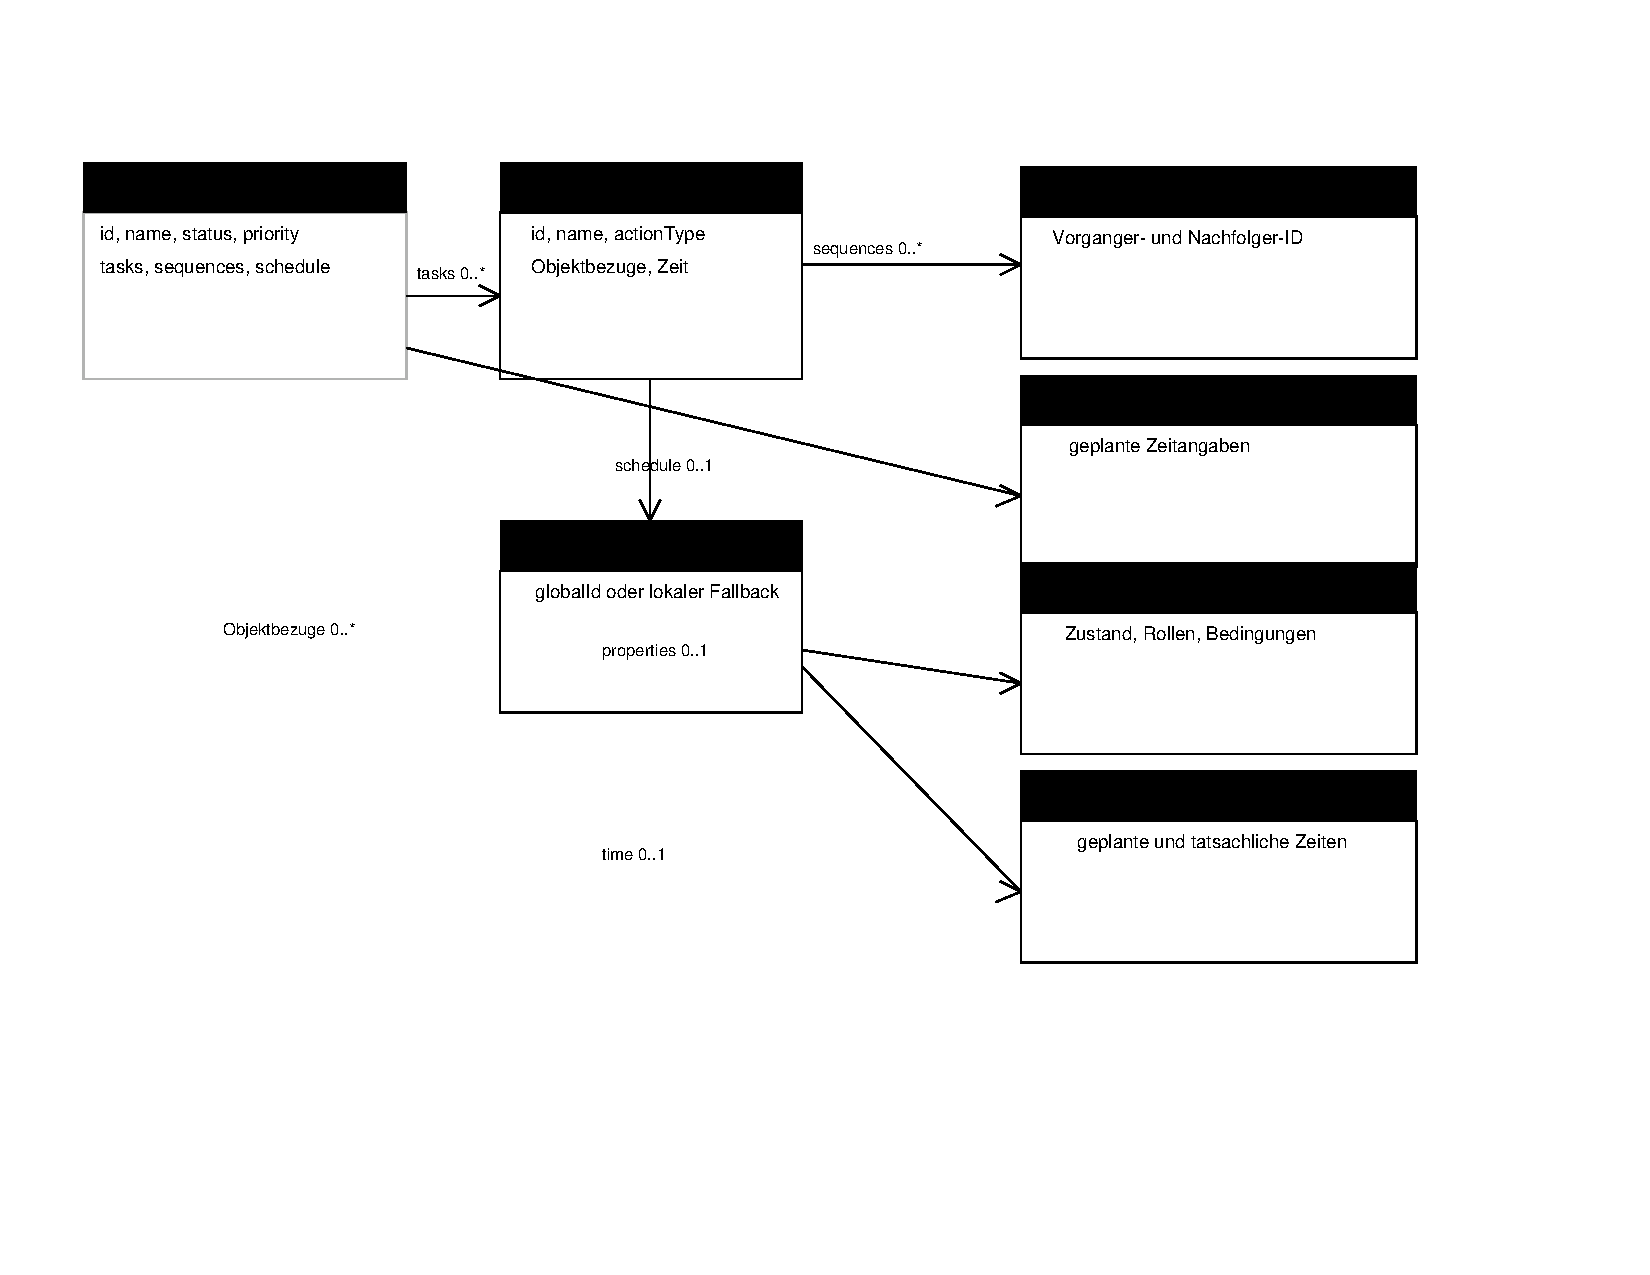
\includegraphics[width=\linewidth]{pics/domain-model-robot-mission.pdf}
  \caption[Internes Domänenmodell für Robotermissionen]{Internes Domänenmodell für Robotermissionen und
  Roboteraufgaben. Eigene Darstellung auf Basis der Implementierung des IFC-Editors am Commit \texttt{674ede3}.}
  \label{fig:domain-model-robot-mission}
\end{figure}

\subsubsection{Zentrale Domänentypen}

\texttt{RobotMission} ist der zentrale fachliche Missionscontainer. Er besitzt eine stabile anwendungsinterne Kennung,
einen Namen sowie optionale Beschreibung, Status- und Prioritätsangaben. Die Felder \texttt{createdAt} und
\texttt{updatedAt} erhalten bei der standardmäßigen Builder-Erzeugung Werte aus \texttt{toISOString()} für die Anlage und
Änderung des Missionswerts. Übergebene Zeitstempelzeichenketten werden dabei nicht auf ihr Format geprüft. Eine Mission
enthält die geordnete Liste \texttt{tasks}, die Liste \texttt{sequences} und optional einen Zeitplan. Neue Missionen werden durch
den Builder zunächst ohne Aufgaben und Sequenzen erzeugt, damit sie als Bearbeitungsentwurf angelegt werden können. Die
abschließende Missionsvalidierung bewertet eine aufgabenlose Mission jedoch als Fehler. Aufgabenkennungen müssen
innerhalb einer Mission eindeutig sein, weil die Sequenzen sie als Endpunkte verwenden.

Eine \texttt{RobotTask} repräsentiert einen abgrenzbaren ausführbaren Schritt innerhalb dieser Mission. Neben Kennung,
Name und optionaler Beschreibung führt sie den projektspezifischen Aktionstyp sowie optionale Status- und
Prioritätswerte. Das am Referenzstand unterstützte Aktionsvokabular umfasst \texttt{OPEN}, \texttt{CLOSE},
\texttt{SWITCH\_ON}, \texttt{SWITCH\_OFF}, \texttt{MOVE}, \texttt{PASS\_THROUGH} und \texttt{NAVIGATE\_TO}. Diese Werte
beschreiben keine IFC-Enumeration. Die Aufgabe trägt außerdem Listen direkter Zielobjekte und indirekt betroffener
Objekte. Für \texttt{MOVE} enthält der Typ davon getrennte Start- und Zielreferenzen. Aufgabenspezifische Änderungs- und
Anlagezeitstempel sind ebenfalls Teil des Typs.

\texttt{RobotObjectReference} beschreibt dabei keine Szene und keine Geometrieinstanz, sondern eine fachliche Referenz
auf ein IFC-Objekt. Bevorzugt wird eine \texttt{globalId}; optional kann sie durch eine \texttt{expressId} für den
Laufzeitzugriff ergänzt sein. Fehlt eine \texttt{globalId}, ist ausschließlich die Kombination aus \texttt{modelId} und
\texttt{expressId} zulässig. Die optionalen Metadaten \texttt{ifcClass} und \texttt{name} dienen der Beschreibung
beziehungsweise der Plausibilitätsprüfung. Damit verbleiben etwa Three.js-Objekte, Fragments-IDs und Rendering-Indizes
außerhalb des fachlichen Modells. Die genaue Persistenz und Auflösung der IFC-Identifikatoren wird in einem späteren
Unterabschnitt behandelt.

\texttt{RobotActionProperties} bündelt die optionalen Angaben zur konkreten Aktion. Dazu gehören ein angestrebter
Zustand, Rollen für Ziel- und betroffene Objekte, eine erforderliche Fähigkeit, Vor- und Nachbedingungen sowie ein
Erfolgskriterium. Diese Eigenschaften sind an \texttt{RobotTask} und nicht an \texttt{RobotObjectReference} gebunden.
Dieselbe Objektreferenz kann somit in unterschiedlichen Aufgaben mit verschiedenen Aktionsanforderungen vorkommen. Die
Semantik der einzelnen Aktionswerte und Parameter wird im folgenden Abschnitt vertieft; an dieser Stelle ist
ausschließlich ihre fachliche Zuordnung zur Aufgabe maßgeblich.

\texttt{RobotTaskTime} fasst optionale Zeitinformationen einer Aufgabe zusammen. Der Typ enthält geplanten Beginn,
geplantes Ende und geplante Dauer ebenso wie tatsächlichen Beginn und tatsächliches Ende, eine geschätzte Restdauer und
einen Fertigstellungsgrad. Der Fertigstellungsgrad ist bei Vorliegen durch die Validierung auf den Wertebereich von 0 bis
1 begrenzt. Die Zeitfelder sind Zeichenketten; eine Formatprüfung auf ISO~8601 ist in der Domänenvalidierung nicht
enthalten. Ihre spätere IFC-Abbildung ist nicht Bestandteil dieses Unterabschnitts. Der Builder übernimmt einen beim
Erzeugen übergebenen optionalen \texttt{RobotMissionSchedule}. Dieser Typ besitzt Kennung und Namen sowie geplanten
Beginn, geplantes Ende und geplante Dauer. Eine eigene Fachvalidierung des Zeitplans ist am Referenzstand nicht
erkennbar.

\texttt{RobotTaskSequence} repräsentiert eine gerichtete Abhängigkeit zwischen zwei Aufgaben derselben Mission. Sie
besitzt eine eigene Kennung, die Kennung der Vorgängeraufgabe, die Kennung der Nachfolgeaufgabe und einen Sequenztyp.
Neben \texttt{FINISH\_START} kennt der Typ \texttt{START\_START}, \texttt{FINISH\_FINISH} und \texttt{START\_FINISH}; beim
Erzeugen einer Sequenz ist \texttt{FINISH\_START} der Standardwert. Eine Sequenz ist keine weitere Hierarchieebene und keine bloße
Sortierinformation. Sie beschreibt vielmehr eine zeitliche Einschränkung zwischen zwei durch ihre stabilen
Aufgabenkennungen bestimmten Schritten.

\subsubsection{Beziehungen und fachliche Grenzen}

Die Aufgabenliste einer Mission erfüllt zwei andere Funktionen als die Sequenzliste. Sie ordnet die untergeordneten
Aufgaben dem Missionscontainer zu und bewahrt eine stabile Darstellungs- beziehungsweise Hierarchiereihenfolge. Aus
dieser Reihenfolge folgt noch keine Ausführungsabhängigkeit. Die Sequenzen bilden einen gerichteten Graphen über
dieselben Aufgaben. Die getrennten Felder \texttt{tasks} und \texttt{sequences} halten Zugehörigkeit, sichtbare
Reihenfolge und Abhängigkeitssemantik daher voneinander getrennt. Für nicht voneinander abhängige Aufgaben verwendet
die implementierte Ordnungsfunktion die Reihenfolge der Aufgabenliste als nachrangiges Ordnungskriterium und erzeugt
dadurch eine deterministische Ordnung. Für einen explizit linearen Ablauf setzt eine weitere Funktion beide Aspekte
bewusst gemeinsam: Sie ersetzt die Sequenzen durch eine \texttt{FINISH\_START}-Kette und ordnet die Aufgabenliste
entsprechend. Beim Löschen einer Aufgabe entfernt der Anwendungsservice zudem alle inzidenten Sequenzen, sodass keine
verwaisten Abhängigkeiten verbleiben.

Bereits die Builder erzwingen nicht leere Missions- und Aufgabenkennungen sowie Namen. Beim Hinzufügen werden doppelte
Aufgaben- und Sequenzkennungen zurückgewiesen; eine neue Sequenz wird außerdem gegen den vollständigen künftigen Graphen
geprüft. Die explizit aufzurufende Domänenvalidierung ergänzt diese Prüfungen um die aufgabenlose Mission, doppelte
Aufgabenkennungen, unbekannte Sequenzendpunkte, Selbstbezüge und Zyklen. Referenzen prüfen nicht leere
\texttt{globalId}-Werte sowie nichtnegative ganzzahlige \texttt{expressId}-Werte; ein lokaler Fallback erfordert eine
\texttt{modelId}. Für Objektinteraktionen verlangt die Validierung die jeweils erforderlichen Referenzen, etwa ein
Zielobjekt für \texttt{OPEN} und \texttt{CLOSE} oder Start- und Zielreferenz für \texttt{MOVE}. Ist eine IFC-Klasse
bekannt und nicht plausibel, wird dies als Fehler gemeldet; fehlende Klasseninformation führt dagegen nur zu einer
Warnung. Ein Domänenwert, der nicht über diese Operationen erzeugt oder anschließend validiert wurde, erfüllt die
genannten Regeln nicht notwendigerweise. Die zugehörigen Domain- und Service-Tests prüfen diese Regeln sowie die
Duplikatbehandlung von Objektbezügen.

Nicht zum Domänenmodell gehören technische Informationen über Three.js-Objekte, Fragments-Modelle, Rendering-IDs oder
den aktuellen UI-Zustand. Ebenso werden \texttt{localStorage}-Schlüssel, Browser-Speichermodi, IFC-Entity-Instanzen,
\texttt{web-ifc}-Laufzeitobjekte, STEP-Serialisierung, Quellbytes und Roundtrip-Provenienz nicht in
\texttt{RobotMission} gespeichert. Die vorhandene Repository-Abstraktion übergibt fachliche Missionswerte; konkrete
Adapter und nachgelagerte IFC-Komponenten verarbeiten die genannten technischen Daten. Dieser Zuschnitt verhindert
insbesondere, dass eine temporäre Auswahl oder eine Speicherimplementierung zum Bestandteil einer fachlichen Aufgabe
wird. Er legt keine Aussage darüber fest, welche Persistenzform künftig verwendet werden muss.

\subsubsection{Zwischenfazit und Überleitung}

Das prototypisch implementierte interne Domänenmodell stellt damit einen prüfbaren fachlichen Bestand für Missionen,
Aufgaben, Objektbezüge, Abhängigkeiten sowie optionale Aktions- und Zeitangaben bereit. Es bereitet eine spätere
Abbildung auf IFC vor, ohne deren Entities oder Serialisierungsdetails in die fachlichen Typen zu übernehmen. Offene
Erweiterungspunkte betreffen insbesondere weitere Aktionsarten und deren Parametrisierung; sie sind am Referenzstand
nicht durch zusätzliche Domänentypen vorweggenommen. Da die konkrete Roboteraktion als Eigenschaft der Aufgabe geführt
wird, untersucht der folgende Abschnitt das verwendete Aktionsvokabular und seine taskbezogene Semantik.
